\documentclass[hidelinks,a4paper]{article}
\usepackage[utf8]{inputenc}
\usepackage[hmargin=2.4cm,vmargin=2.4cm]{geometry}
\usepackage{amsfonts}
\usepackage{amsmath,amsthm,amssymb}
\usepackage{polski}
\usepackage{ulem}

\usepackage[cache=false]{minted}

\setminted[python]{
    breaklines=true,
    mathescape=true,
    escapeinside=||,
    encoding=utf8
}

\usepackage{tikz}
\usetikzlibrary{snakes}

\setlength{\parindent}{0em}
\setlength{\parskip}{0.4em}

\usepackage{longtable}

\title{Numerki}

\newcommand{\II}{\mathbb{I}}
\newcommand{\RR}{\mathbb{R}}
\newcommand{\EE}{\mathbb{E}}
\newcommand{\CC}{\mathbb{C}}
\newcommand{\ra}{\rightarrow}
\newcommand{\la}{\leftarrow}
\newcommand{\pl}{\parallel}
\newcommand{\eye}{I}

\newcommand{\norm}[1]{\left\lVert#1\right\rVert}

\newtheorem{wniosek}{Wniosek}
\newtheorem{defi}{Definicja}
\newtheorem{fakt}{Fakt}
\newtheorem{lemat}{Lemat}
\newtheorem{twierdz}{Twierdzenie}

\usepackage{ wasysym }
\usepackage{ marvosym }
\usepackage{dirtytalk}



\begin{document}
\linespread{1.0}
\maketitle

\tableofcontents

\clearpage

\section*{Info na start}

\begin{itemize}
	\item 10p. aktywność na ćwiczeniach (pewnie prace domowe)
	\item 20p. lab
	\item 20p. kolos 23.XI. na wykładzie
	\item 50p. egzamin
\end{itemize}

Ocena: $max(K + L + C + E, 2 \cdot E - 5)$

I termin: $K + L + C > 20p$

G. Stewart "Afternotes on numerical analysis"

\section{Układy równań liniowych}

$x \in \RR^N$

$A \in \RR^{N,N}, \textrm{nieosobliwa}$

$b \in \RR^N$

\[
	A \cdot x = b
\]

\subsection{Proste układy równań}

\subsubsection{Macierze trójkątne}

$
\left\{
\begin{array}{ll}
	a_{11}x_1                                  & = b_1 \implies x_1 = \cfrac{b_1}{a_{11}}                \\
	a_{21}x_1 + a_{22}x_2                      & = b_2 \implies x_2 = \cfrac{1}{a_{22}}(b_2 - a_{11}x_1) \\
	\vdots \\
	a_{m1}x_1 + a_{m2}x_2 + \cdots + a_{mn}x_n & = b_n                                                   
\end{array}
\right.
$

$x_n = \cfrac{1}{a_{nk}}(b_k - \sum_{j=1}^{k-1} a_{kj}x_j)$

Gdy macierz układu ma formę trójkątną, to koszt wyznaczenia rozwiązania:

\[
	\left[
		\begin{array}{ccccc}
			a_{0,0} \\
			a_{0,1} & a_{1,1}  &   & \text{\huge0}\\
			a_{0,2}  & a_{1,2} & a_{2,2} \\
			\vdots  & \vdots & \vdots & \ddots \\
			a_{0,n} & a_{1,n} & \cdots & a_{n-1,n} & a_{n,n} 
		\end{array}
	\right]
	\cdot
	\left [
		\begin{array}{c}
			x_1 \\  \vdots \\  \vdots \\ x_n
		\end{array}
	\right]
	=
	\left [
		\begin{array}{c}
			b_1 \\ \vdots \\ \vdots \\ b_n
		\end{array}
	\right]
\]

to

\begin{align*}
	x_0 & = \frac{b_0}{a_{0,0}}                                & \text{(jedna operacja)}    \\
	x_1 & = \frac{b_1 - a_{0,1} x_0}{a_{1,1}}                  & \text{(trzy operacje)}     \\
	&\vdots \\
	x_n & = \frac{b_n - \sum_{i=0}^{n-1} a_{i,n} x_i}{a_{n,n}} & \text{($2n + 1$ operacji)} 
\end{align*}

A koszt rozwiązania jest następujący:
$1+3+5+...+2(k-1)+1+... = \sum_{k=1}^{n} 2k - \sum 1 = O(2n^2)$

Jest to metoda podstawienia w przód/tył. Rozmiar danych jest rzędu $O(n^2)$, więc widać, że to jest optymalna metoda.

\subsubsection{Macierze ortogonalne}

Gdy mamy macierz ortogonalną, tzn.

$Q^T \cdot Q = I$, gdzie $Q \in \RR^{N, N}$

$\arraycolsep=0.6em\def\arraystretch{1.8}
\left[
	\begin{array}{c}
		\quad _1^T \quad   \\ \hline
		\quad q_2^T \quad  \\ \hline
		\quad \vdots \quad \\ \hline
		\quad q_n^T \quad  
	\end{array}
\right]
\cdot
\left[
	\begin{array}{c|c|c|c}
		    &     &        &     \\
		q_1 & q_2 & \cdots & q_n \\
		    &     &        &     
	\end{array}
\right]
=
\left[
	\begin{array}{cccc}
		1 &   &        & 0 \\
		  & 1 &        &   \\
		  &   & \ddots &   \\
		0 &   &        & 1 
	\end{array}
\right]	
$

Jej kolumny są wzajemnie prostopadłe o normie euklidesowej równej $1$. Nie trudno zauważyć, że zachodzi też $Q \cdot Q^T = \eye$.

Układ $Q \cdot x = b$ ma rozwiązanie:
\begin{equation}
	\begin{aligned}
		Q \cdot x           & = b           \\
		Q^T \cdot Q \cdot x & = Q^T b       \\
		x                   & = Q^T \cdot b \\
	\end{aligned}
\end{equation}

koszt to koszt wymnożenia macierzy, zatem  $O(n^2)$.


\subsection{W miarę proste układy równań}

\subsubsection{Układ z łatwym blokiem}

Przypuśćmy, że nasz układ jest postaci blokowej

$\arraycolsep=1em\def\arraystretch{2}
\left[
	\begin{array}{c|c}
		A_1 & E \\ \hline
		B   & C 
	\end{array}
\right] \cdot
\left[
	\begin{array}{c}
		x \\ \hline
		y 
	\end{array}
\right] = 
\left[
	\begin{array}{c}
		f \\ \hline
		g 
	\end{array}
\right]
$

gdzie A, B, C, E to macierze, układy z A potrafimy ``łatwo" rozwiązać.

\[
	\left\{ \begin{array}{l}
	A_1x + Ey = f\\
	Bx + Cy = g
	\end{array} \right.
\]

\[
	\left\{ \begin{array}{l}
	A_1x = f - Ey\\
	Bx + Cy = g
	\end{array} \right.
\]


\[
	\left\{ \begin{array}{l}
	x = A_1^{-1}(f - Ey)\\
	Bx + Cy = g
	\end{array} \right.
\]

\[
	B \cdot A_1^{-1} (f - Ey) + Cy = g \implies (C - BA_1^{-1}E)y = g - B\cdot A_1^{-1}f
\]

\textbf{Algorytm}:

\begin{enumerate}
	\item Rozwiąż układ równań $A_1w = f$
	\item Rozwiąż układ $A_1 \cdot G = E$
	\item Rozwiąż $(C-FG)y = y - Fw$ (jeśli potrafisz)
	\item $x = w - Gy$
\end{enumerate}


\subsubsection{Układy ze znanym rozkładem macierzy}

Załóżmy, że $A = B_1 \cdot B_2$, gdzie macierze $B_1$, $B_2$ są "łatwe". Wtedy układ $A\cdot x = b$ też jest łatwy.

$B_1 \cdot \underbrace{ B_2 \cdot x}_{y} = b$

\textbf{Algorytm}:

\begin{enumerate}
	\item Rozwiąż $B_1 y = b$
	\item Rozwiąż $B_2 x = y$
\end{enumerate}

\subsubsection{}

Zauważmy, że na ten algorytm można popatrzeć jak na rozkład na "łatwiejsze" macierze

\[\arraycolsep=1em\def\arraystretch{2}
	\left[
		\begin{array}{c|c}
			A_1 & E \\ \hline
			F   & C 
		\end{array}
	\right] =
	\left[
		\begin{array}{c|c}
			\eye     & 0 \\ \hline
			F A^{-1} & I 
		\end{array}
	\right]
	\cdot 
	\left[
		\begin{array}{c|c}
			A_1 & E \\ \hline
			0   & S 
		\end{array}
	\right]
\]

Gdzie $S = C - FG = C - FA^{-1}E$


\textbf{Pomysł}: znaleźć rozkład macierzy A na iloczyn macierzy dolnej i górnej trójkątnej.

\[
	A = \underbrace{\left[
			\begin{array}{cc}
				      & 0 \\
				\star &   
			\end{array}
		\right]}_{L} \cdot
	\underbrace{\left[
			\begin{array}{cc}
				  & \star \\
				0 &       
			\end{array}
		\right]}_{U}
\]

Spróbujmy blokowo:

\[\arraycolsep=0.7em\def\arraystretch{1.4}
	\left[
		\begin{array}{c|c}
			A_{11} & A_{12} \\ \hline
			A_{21} & A_{22} 
		\end{array}
	\right] =
	\left[
		\begin{array}{c|c}
			L_{11} & 0      \\ \hline
			L_{21} & L_{22} 
		\end{array}
	\right]
	\cdot 
	\left[
		\begin{array}{c|c}
			L_{11} & L_{12} \\ \hline
			0      & L_{22} 
		\end{array}
	\right]
\]

Mnożąc dostajemy:

$
\begin{array}{ll}
	A_{1,1} & = L_{1,1} \cdot U_{1,1}                                                                           \\
	A_{2,1} & = L_{2,1} \cdot U_{1,1} \implies L_{2,1} = A_{2,1}U_{11}^{-1}                                     \\
	A_{1,2} & = L_{1,1} \cdot U_{1,2}  \implies U_{1,2} = L^{-1}_{1,1} A_{1,2}                                  \\
	A_{2,2} & = L_{2,1} \cdot U_{1,2} + L_{1,2} \cdot A_{2,2} \implies A_{22} - L_{2,1}U_{1,2} = L_{2,2}U_{2,2} 
\end{array}
$

Mamy rekurencyjny algorytm rozkładu $LU$, ale w klasycznym przypadku biorąc podział blokowy można uniknąć rekurencji.

\[\arraycolsep=0.7em\def\arraystretch{1.4}
	\begin{array}{l}
		\updownarrow 1   \\ \\
		\updownarrow N-1 \\ \ 
	\end{array}
	\left[
		\begin{array}{c|c}
			a_{11} & \quad a_{12}^T \quad \\ \hline & \\
			a_{21} & A_{22}               \\ &
		\end{array}
	\right] =
	\left[
		\begin{array}{c|c}
			q      & \quad 0^T \quad \\ \hline & \\
			l_{21} & L_{22}          \\ &
		\end{array}
	\right]
	\cdot 
	\left[
		\begin{array}{c|c}
			u_{11} & \quad u_{12}^T \quad \\ \hline & \\
			0      & U_{22}               \\ &
		\end{array}
	\right]
\]

$L_{1,1} = 1$, $u_{1,1} = a_{1,1}$

$L_{2,1} = \frac{1}{a_{1,1}} \cdot a_{?}$

$\underbrace{\tilde{A}_{22} - L_{21}U_{12}^T}_{\textrm{wystarczy rozłożyć taką macierz - stąd algorytm iteracyjny}} = L_{22} \cdot U_{22}$


Można na to patrzeć jako na sekwencję przejść A prowadzącą do macierzy U. A to jest tak naprawdę eliminacja Gaussa.

\subsection{Algorytm eliminacji Gaussa}

Ten algorytm nie zadziała jeśli w trakcie będziemy dzielić przez 0, np.

$A = \left[
	\begin{array}{cc}
		0 & 1 \\
		1 & 0 
\end{array}\right]$ (nieosobliwa)
    
Aby algorytm eliminacji Gaussa zadziałał zawsze (o ile tylko A - nieosobliwa), uzupełnimy go o procedurę \uwave{wyboru elementu głównego} (osiowania). 

\begin{enumerate}
	\item Szukamy w kolumnie, w której prowadzimy eliminację, elementu  największym module (niezerowy, bo A nieosobliwa)
	\item "Zamieniam"\footnote{Zamiana wierszy - mnożenie macierzy przez macierz permutacji} wiersz, w którym jest znaleziony element z wierszem wyżej 
\end{enumerate}


\begin{wniosek} Algorytm eliminacji Gaussa z wyborem elementu głównego w kolumnie prowadzi do rozkładu
	
	\[
		P \cdot A = L \cdot U
	\]
	gdzie $P$ to macierz permutacji, $L$ - dolna trójkątna, $U$ - górna trójkątna.
	
\end{wniosek}

Stąd algorytm rozwiązywania układów równań:

\begin{enumerate}
	\item Rozłóż $PA = LU$
	\item Rozwiąż $Ly= Pb$ $\quad\quad O(n^2)$
	\item Rozwiąż $Ux = y$ $\quad\quad O(n^2)$
\end{enumerate}

Koszt rozkładu:

$2*(n-1)^2 + 2(n-2)^2 + ... + 2 + O(n^2) = 2 \cdot \underbrace{((n-1)^2 + (n-2)^2 + ... + 1^2)}_{\frac{1}{3}n^2}$


\section{Liczby zmiennopozycyjne i arytmetyka}

\[
	\underbrace{6,63}_{mantysa} \cdot \underbrace{10^{\overbrace{-34}^{wykładnik}}}_{\textrm{rząd wielkości}}
\]

Liczby maszynowe:

$x = (-1)^{\overbrace{s}^{\textrm{znak}}} \cdot \underbrace{m}_{\textrm{mantysa}} \cdot \underbrace{\beta^{\overbrace{e}^{\textrm{wykładnik}}}}_{\textrm{podstawa - u nas 2}}$

$0 \leq m < \beta$

$e - \textrm{wykładnik, liczba całkowita taka, że } 0 > e_{min} \leq e \leq e_{max} > 0$

Charakterystyka zestawu: $(\beta, \underbrace{e_{min}, e_{max}}_{zakres}, \underbrace{p}_{precyzja})$

\subsection{Liczby znormalizowane}

\[
	x = (-1)^s \cdot m \cdot 2^e
\]

ale zakładamy, że m jest postaci (a więc $1 \leq m < 2)$

\[
	m = (1.f_1,f_2,f_3,...)
\]

To daje jednoznaczną reprezentację liczb niezerowych. Dodatkowo $f_0$ nie trzeba pamiętać w pamięci komputera.

\subsection{Standard arytmetyki zmiennopozycyjnej}

$\underbrace{\textrm{IEEE-754}}_{Kahan} \rightarrow \textrm{IEEE-854} \rightarrow \underbrace{\textrm{IEEE-754-R}}_{e_{min} = 1 - e_{max}}$

W pamięci komputera przechowujemy:

\begin{tabular}{|c|c|l|l|l|c|c|c|l|c|}
	\hline
	s & \multicolumn{4}{c|}{e + bias} & $f_1$ & $f_2$ & \multicolumn{2}{c|}{...} & $f_{p-1}$ \\ \hline
\end{tabular}


\begin{longtable}[c]{l|l|l|l|l|l|l}
	nazwa               & p   & $e_{min}$ & $e_{max}$ & size & bias  & nazwa IEEE-754-R \\ \hline
	\endfirsthead
	%
	\endhead
	%
	single precision    & 24  & -126      & +127      & 32   & 127   & binary32         \\ \hline
	double precision    & 53  & -1022     & +1023     & 64   & 1023  & binary64         \\ \hline
	double extended     & 64  & -16382    & +16383    & 80   & 16383 &                  \\ \hline
	half precisision    & 11  & -14       & 15        & 16   & 15    & binary16         \\ \hline
	quadruple precision & 113 & -16382    & +16383    & 128  & 16383 & binary128        
\end{longtable}

\begin{tabular}{|c|c|l|l|l|c|c|c|l|c|}
	\hline
	0 & \multicolumn{4}{c|}{0...0} & 0 & 0 & \multicolumn{2}{c|}{...} & 0 \\ \hline
\end{tabular} = $+0.0$

\begin{tabular}{|c|c|l|l|l|c|c|c|l|c|}
	\hline
	1 & \multicolumn{4}{c|}{0...0} & 0 & 0 & \multicolumn{2}{c|}{...} & 0 \\ \hline
\end{tabular} = $-0.0$

\begin{tabular}{|c|c|l|l|l|c|c|c|l|c|}
	\hline
	0 & \multicolumn{4}{c|}{1...1} & 0 & 0 & \multicolumn{2}{c|}{...} & 0 \\ \hline
\end{tabular} = $+\infty$

\begin{tabular}{|c|c|l|l|l|c|c|c|l|c|}
	\hline
	1 & \multicolumn{4}{c|}{1...1} & 0 & 0 & \multicolumn{2}{c|}{...} & 0 \\ \hline
\end{tabular} = $-\infty$

\begin{tabular}{|c|c|l|l|l|c|c|c|l|c|}
	\hline
	0 & \multicolumn{4}{c|}{1...1} & niezero \\ \hline
\end{tabular} = NaN

np. $\frac{0}{0} = \infty - \infty = NaN$

\subsection{Zabawkowy system fl (floating point)}

(bez biasu)

$\beta = 2$, $p = 3$, $e_{min} = -1, e_{max} + 1$

$x = (1.f_1f_2)_2 \cdot 2^{e}$

\begin{tikzpicture}[snake=zigzag, line before snake = 5mm, line after snake = 5mm]
	% draw horizontal line
	\draw [->] (0,0) -- (16,0);
	
	% draw vertical lines
	\foreach \x in {1, 5, 9, 13}
	\draw (\x cm,6pt) -- (\x cm,-6pt);
	
	\foreach \x in {3, 3.5, 4, 4.5, 6, 7, 8, 11, 15}
	\draw (\x cm,3pt) -- (\x cm,-3pt);
	
	% draw nodes
	\draw (1,0) node[below=6pt] {$ 0 $};
	\draw (3,0) node[below=6pt] {$ \frac{1}{2} $};
	\draw (5,0) node[below=6pt] {$ 1 $};
	\draw (9,0) node[below=6pt] {$ 2 $};
	\draw (13,0) node[below=6pt] {$ 3 $};
\end{tikzpicture}


Aby wypełnić pustkę wokół zera uzupełnia się system o liczby subnormalizowane:

\[
	(0.f_1f_2...f_{p-1})_2 \cdot 2^{e_{min}}
\]

Reprezentacja liczb rzeczywistych w arytmetyce fl:

\[
	x \in \mathbb{R} \rightarrow fl(x) : \textrm{jego numeryczna reprezentacja (l. masyznowa odpowiadjąca x)}
\]

Gdy x - liczba maszynowa, fl(x) = x.

Jeśli nie, to

\[
	fl(x) = Round(x)
\]

Gdzie $Round(x)$ może być wybrany na jeden ze sposobów:

\begin{enumerate}
	\item $RN(x)$ - zaokrąglenie do najbliższej liczby maszynowej (domyślne)
	\item $RD(x)$ - zaokrąglenie w dół (tzn. w stronę $-\infty$
	\item $RU(x)$ - zaokrąglenie w górę (tzn. w stronę $\infty$)
	\item $RZ(x)$ - zaokrąglenie w stronę zera
\end{enumerate}

Dalej zakładamy, że $fl(x) = RN(x)$. Wtedy łatwo pokazać, że 
\[
	\frac{|fl(x) - x|}{|x|} \leq 2^{-p} = \nu \leftarrow \textrm{ preycja arytmetyki}
\]

(o ile nie ma undeflow/overflow)

Inaczej mówiąc:

\[
	fl(x) = x(1 + \varepsilon), |\varepsilon| \leq \nu
\]

---

\[
	a\ \square\ b\ \textrm{jest równy} fl(a\ \square\ b)\textrm{, gdzie }\square \in \{+, -, \times, :\}
\]

co zapisujemy

\[
	\underbrace{fl(a\ \square\ b)}_{\textrm{wynik w fl}} = \underbrace{fl(a\ \square\ b)}_{\textrm{reprezentacja} a \square b \textrm{ w fl}}
\]

(o ile brak underflow/overfow/NaN)

Ponadto tak też ma być dla $\sqrt{}$ i dla

\[
	\underbrace{FMA(a, b, c)}_{\textrm{fast multiply add}} := a \cdot b + c
\]

$fl(FMA(a, b, c) = fl(a \cdot b + c)$

\subsection{Problemy arytmetyki fl}

Źródła błędu algorytmu rozwiązującego zadanie:
\begin{itemize}
	\item reprezentacja danych w fl
	\item reprezentacja wyniku w fl
	\item realizacja algorytmu w fl
\end{itemize}


\subsubsection{Redukcja cyfr przy odejmowaniu}

Dane: $x, y \in \RR$. Obliczamy
\[
	s := x + y
\]

\begin{enumerate}
	\item Reprezentacja danych: $\tilde{x} = fl(x) = x(1+\varepsilon)$,
	      $\tilde{y} = fl(y) = y(1 + \varepsilon)$
	\item Wykonanie algorytmu
	      \[
	      	\tilde{s} = fl(\tilde{x} + \tilde{y}) = (\tilde{x} + \tilde{y})(1 + \varepsilon)
	      \]
\end{enumerate}

Jaki jest błąd?

\[
	\cfrac{|\tilde{s} - s|}{|s|} = \cfrac{|x + (\varepsilon_x + \varepsilon)\cdot x + y + (\varepsilon_y + \varepsilon)\cdot y + \textrm{małe }\nu^2|}{|x + y|} \leq \cfrac{}{} \leq 2 \cdot \cfrac{|x|+|y|}{|x+y|} \cdot \nu
\]

Zatem

- jeśli $x \simeq -y$, to $2\cfrac{|x|+|y|}{|x+y|} \gg 1$. Czyli błąd względny może być bardzo duży.

- jeśli $x, y$ - tego samego znaku, to $2 \cfrac{|x|+|y|}{|x+y|} = 2 \cfrac{|x+y|}{|x+y|} = 2$. Czyli błąd względny na poziomie $\nu$.

\subsubsection{Błędy w obliczeniach numerycznych}

Zadanie obliczeniowe: $P: \RR^n \supset D \ra \RR^n$. Mając dane $x \in D$ (dziedzina), wyznaczyć $y = P(x)$.

Dane:

\begin{enumerate}
	\item Dane: $x \in \RR$. Obliczyć $y=\sin(x)$.
	\item Dane: $A \in \RR^{N \times N}$, $x \in \RR^n$. Obliczyć $y = A \cdot b$.
	      $D = \RR^{N \times N} \times R^N$
	\item Dane $A \in \RR^{N \times N}$, $b \in \RR^n$. Obliczyć rozwiązanie układu $Ay = b$. Wtedy $P(x) := A^{-1}x$
	\item Dla danego $F: \RR \ra \RR$ obliczyć $x$, t. że $f(x) = 0$
	      $P(z) = f^{-1}(z)$, $D = \{0\}$
\end{enumerate}


\subsection{Błąd względny i bezwzględny}
$x \in \RR^n$ - dokładna wartość

$\tilde{x} \in \RR^n$ - wartość przybliżona

błąd bezwzględny - $\parallel \tilde{x} - x \parallel$

błąd względny - $\cfrac{\textrm{błąd bezwzględny}}{\parallel x \parallel}$

{\centering 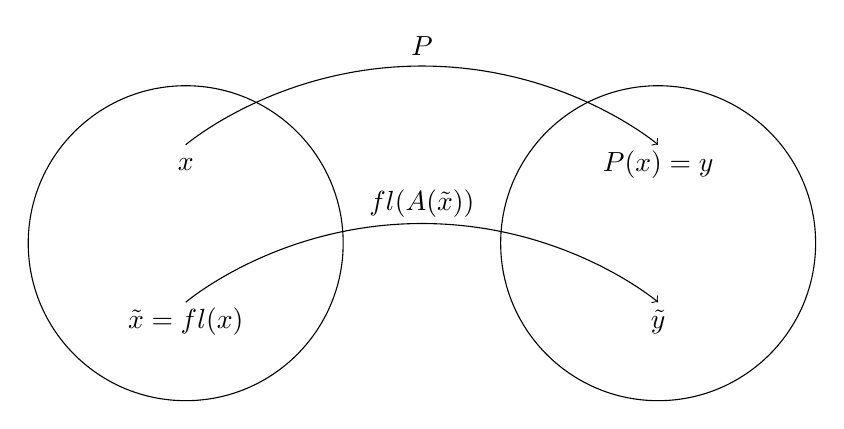
\begin{tikzpicture}
	\draw  (-3,0) ellipse (2 and 2);
	\draw  (3,0) ellipse (2 and 2);
	
	\draw  [->] plot[smooth, tension=1.1] 
	   coordinates {(-3,1.25) (0,2.25) (3,1.25)};
	\node at (-3,1) {$x$};
	\node at (3,1) {$P(x)=y$};
	\node at (0,2.5) {$P$};
	
	\draw  [->] plot[smooth, tension=1.1] 
	   coordinates {(-3,-0.75) (0,0.25) (3,-0.75)};
	\node at (-3,-1) {$\tilde{x} = fl(x)$};
	\node at (3,-1) {$\tilde{y}$};
	\node at (0,0.5) {$fl(A(\tilde{x}))$};
\end{tikzpicture}\par}

{\centering 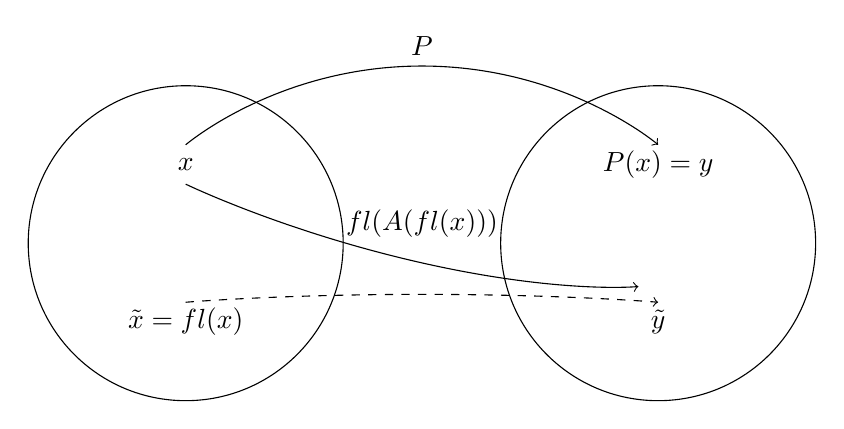
\begin{tikzpicture}
	\draw  (-3,0) ellipse (2 and 2);
	\draw  (3,0) ellipse (2 and 2);
	
	\draw  [->] plot[smooth, tension=1.1] 
	   coordinates {(-3,1.25) (0,2.25) (3,1.25)};
	\node at (-3,1) {$x$};
	\node at (3,1) {$P(x)=y$};
	\node at (0,2.5) {$P$};
	
	\draw  [dashed] [->] plot[smooth, tension=1.1] 
	   coordinates {(-3,-0.75) (0,-0.65) (3,-0.75)};
	\node at (-3,-1) {$\tilde{x} = fl(x)$};
	\node at (3,-1) {$\tilde{y}$};
	\node at (0,0.25) {$fl(A(fl(x)))$};
	
	\draw  [->] plot[smooth, tension=1.1] 
	   coordinates {(-3,0.75) (0,-.25) (2.75,-0.55)};
\end{tikzpicture}\par}

\begin{defi}[Silnie numeryczna poprawność]
	Algorytm A jest \textbf{silnie numerycznie poprawny (NP)} jeśli $\tilde{y} = P(\tilde{x})$ - dokładny wynik dla trochę zaburzonych danych, gdzie $\frac{\parallel \tilde{x} - x\parallel}{\parallel x \parallel} \leq \underbrace{k}_{\textrm{nieduża stała}} \cdot \nu$
\end{defi}

\begin{defi}[Numeryczna poprawność]
	Algorytm m jest \textbf{numerycznie poprawny}, jeśli jego wynik możemy zinterpretować jako prawie dokładne rozwiązanie na prawie dokładnych danych.
	
	$c\frac{\parallel \tilde{x} - x \parallel}{\parallel x + y \parallel} \leq k \cdot \nu$ (prawie dokładne dane)
	
	$\cfrac{\parallel \tilde{y} - P(\tilde{x}) \parallel}{\parallel P(x) \parallel} \leq k \cdot \nu$ (prawie dokładny wynik)
	
\end{defi}

{\centering 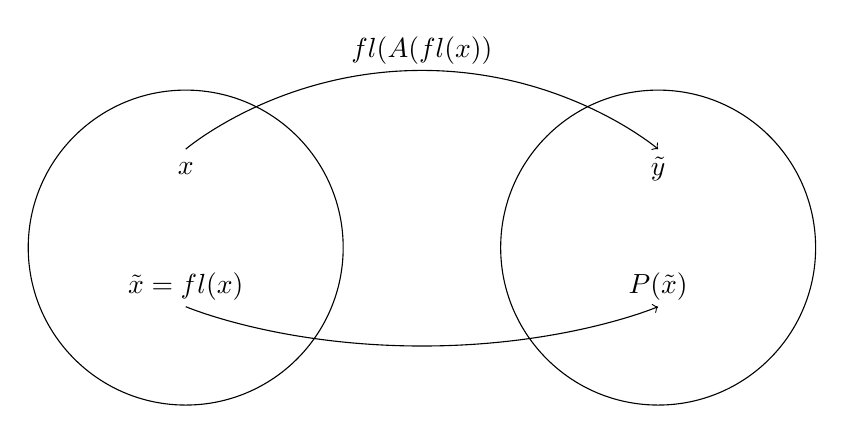
\begin{tikzpicture}
	\draw  (-3,0) ellipse (2 and 2);
	\draw  (3,0) ellipse (2 and 2);
	
	\draw  [->] plot[smooth, tension=1.1] 
	   coordinates {(-3,1.25) (0,2.25) (3,1.25)};
	\node at (-3,1) {$x$};
	\node at (3,1) {$\tilde{y}$};
	\node at (0,2.5) {$fl(A(fl(x))$};
	
	\draw  [->] plot[smooth, tension=1.1] 
	   coordinates {(-3,-0.75) (0,-1.25) (3,-0.75)};
	\node at (-3,-0.5) {$\tilde{x} = fl(x)$};
	\node at (3,-0.5) {$P(\tilde{x})$};
\end{tikzpicture}\par}

\begin{defi}[Polityczna poprawność]\end{defi}

\subsection{Uwarunkowanie zadania (czułość zadania na zaburzenia)}

Pytanie: jak dobrym przybliżeniem $P(x)$ jest y? 

$\cfrac{\norm{P(x) - P(\tilde{x})}}{\norm{P(x)}} = \cfrac{\norm{P(X) < y}}{\norm{P(x)}} \leq ?$

To jest pytanie o czułość zadania P na zaburzenia danych i nie ma nic wspólnego z tym jaki algorytm użyjemy.


Zamiast iksa biorę iks zaburzony. Pytanie jaki jest błąd (Względny):

\[
	\cfrac{\parallel P(x + \delta) - P(x) \parallel}{\parallel P(x) \parallel} \leq ? \cdot \frac{\norm{\delta}}{\norm{x}}
\]

(błąd względny wyniku vs zaburzenie względne danych)

Lub bezwzględny (błąd bezwzględny wyniku)


\begin{defi}
	Wskaźnik (wspólczynnik) uwarunkowania zadania P w punkcie x
	
	\[
		cond_{abs}(P, x) := sup_{\delta\textrm{ dost. małe}}\left(\frac{\norm{P(x + \delta) - P(x)}}{\norm{\delta}}\right)
	\]
	
	wtedy (dla tych $\delta$):
	
	\[
		\norm{P(x + \delta) - P(x)} \leq cond_{abs} (P, x) \cdot \norm{\delta}
	\]
	
	Analogicznie:
	
	\[
		cond_{rel}(P, x) := sup_{\delta\textrm{ dost. małe}}\left(\frac{\norm{P(x + \delta) - P(x)} \cdot \norm{x}}{\norm{\delta} \cdot \norm{P(x)}}\right)
	\]
	
	wtedy dla tych $\delta$:
	
	\[
		\frac{\norm{P(x + \delta) - P(X)}}{\norm{P(x)}} \leq cond_{rel} (P, x) \frac{\norm{\delta}}{\norm{x}}
	\]
	
\end{defi}

\textbf{IDEALIZACJA}: uwarunkowanie w punkcie (tzn. gdy $\delta \ra 0$):

\[\def\arraystretch{3.4}
	\begin{array}{ll}
		cond_{abs}(P, x) & := \lim_{\norm{\delta} \ra 0} \cfrac{\norm{P(x + \delta) - P(x)}}{\norm{\delta}} \\
		cond_{rel}(P, x) & := \lim_{\norm{\delta} \ra 0} \cfrac{\norm{P(x + \delta) - P(x)} \cdot \norm{x}}{\norm{\delta} \cdot \norm{P(x)}} \\ & = cond_{abs} (P, x) \cdot \cfrac{\norm{x}}{\norm{P(x)}}
	\end{array}
\]

\textbf{PRZYKŁAD}:

$P(x) = f(x) \in \RR, x \in R$

$cond_{abs} (P, x) = cond_{abs}(f, x) = \lim_{| \delta | \ra 0} \cfrac{| f(x + \delta) - f(x)|}{| \delta |} = |f'(x)|$

$cond_{rel}(P, x) = \cfrac{|f'(x)| \cdot |x|}{|f(x)|}$

Powiemy, że zadanie P jest źle uwarunkowane w punkcie x, jeśli:
\[
	cond(P, x) \gg 1
\]
Wtedy małe zaburzenie danych może spowodować duży błąd wyniku. W przeciwnym razie mówimy, że zadanie jest dobrze uwarunkowane.

\begin{wniosek} Algorytm NP w zadaniu dobrze uwarunkowanym musi dawać wynik obarczony małym błędem. \end{wniosek}

\subsubsection{Uwarunkowanie układu równań liniowych}


$x = A^{-1}b, Ax = b$

$\tilde{x} = A^{-1}(b + \delta) = A\tilde{x} = b + \delta$, $\frac{pl x - \tilde{x} \norm{}{} x pl} \leq ?$


$\frac{\norm{\delta}}{\norm{b}} \leq \varepsilon$

\[
	\norm{x - \tilde{x}} = \norm{A^{-1}b - A^{-1}(b + \delta)} = \norm{A^{-1}b - A^{-1}b - A^{-1}\delta} \leq \pl A
\]


\[
	\frac{\norm{x - \tilde{x}}}{\norm{x}} \leq \frac{\norm{A^{-1}} \cdot \norm{\delta}}{\norm{x}} = \frac{\norm{A^{-1}} \cdot \norm{\delta} \cdot \norm{b}}{\norm{x} \cdot \norm{b}} \leq \frac{\norm{A^{-1}} \cdot \norm{b}}{\norm{x}} \cdot \varepsilon = \frac{\norm{A^{-1}} \cdot \norm{Ax}}{\norm{x}} \cdot \varepsilon \leq \underbrace{\norm{A} \cdot \norm{A^{-1}}}_{cond(A)} \cdot \varepsilon
\]

Wpływ zaburzeń macierzy i prawej strony:

$Ax = b$, $(a + \Delta)\tilde{x} = b + \delta$, gdzie

$\frac{\norm{\Delta}}{\norm{A}} \leq \varepsilon$, $\frac{\delta}{b} \leq \varepsilon$

Okazuje się, że jeśli:

\[
	\varepsilon \norm{A} \cdot \norm{A^{-1}} \leq \frac{1}{2}
\]

to

\[
	\frac{\norm{x - \tilde{x}}}{\norm{x}} \leq 4 \cdot cond(A) \cdot \varepsilon
\]

Dowód:

$(A + \Delta)\tilde{x} = Ax + \delta$

stąd

$A(\tilde{x} - x) = \delta - \Delta \tilde{x} = \delta - \Delta(\tilde{x} - x) - \Delta x$

$(A+\Delta)(\tilde{x} - x) = \delta - \Delta \cdot x$

$\norm{\tilde{x} - x} = \norm{(A+\Delta)^{-1}(\delta - \Delta x)} \leq \norm{(A + \Delta)^{-1}} \cdot \norm{\delta - \Delta}$

\begin{lemat} Jeśli $\norm{B} < 1$, to macierz $I + B$ jest odwracalna oraz
	\[
		\norm{(I + B)^{-1}} \leq \frac{1}{1 - \norm{B}}
	\]
\end{lemat}

\begin{proof}
	Gdyby była osobliwa, to $\exists x \neq 0$
	    
	\[
		(I + B)x = 0
	\]
	    
	\[
		x + Bx = 0
	\]
	    
	$\norm{x} = \norm{-Bx} = \norm{Bx} \leq \norm{B} \cdot \norm{x}$
	    
	\[
		1 \leq \norm{B}
	\]
	    
	sprzeczność.
\end{proof}

\begin{wniosek} Jeśli $A$ jest odwracalna i $\norm{A ^ {-1} \Delta} < 1$, to $(A + \Delta)^{-1}$ istnieje i rzecz jasna
	\[
		(A \cdot \Delta)^{-1} \leq \frac{\norm{A^{-1}}}{1 - \norm{A^{-1}} \cdot \underbrace{\norm{\Delta}}_{\leq \varepsilon \cdot \norm{A}}}
	\]
	
	$A + \Delta  A(I + A^{-1} \Delta)$
	
	Zatem
	
	\[
		\norm{\tilde{x} - x} \leq \frac{\norm{A^{-1}}}{1 - \varepsilon \norm{A^{-1}} \cdot \norm{A}} \leq ... \leq \frac{2 \cdot \norm{A^{-1}} \cdot \norm{A}}{1 - \varepsilon \norm{A^{-1}} \cdot \norm{A}} \cdot \norm{x} \cdot \varepsilon
	\]
\end{wniosek}

\begin{fakt} Algorytm rozwiązywania układu $Ax = b \in \RR^n$ przez rozkład LU z wyborem w kolumnie (eliminacja Gaussa z wyborem w kolumnie) produkuje w fl rozwiązanie $\tilde{x}$ takie, że $\tilde{x}$ spełnia (dokładnie) rozwiązanie:
	
	\[
		(A + \Delta)\tilde{x} = b
	\]
	
	gdzie
	
	\[
		\frac{\norm{\Delta}_\infty}{\norm{A}_\infty} \leq \underbrace{K}_{\textrm{nieduża stała}} \cdot N^3 \cdot \overbrace{\rho_N}^{\textrm{wskaźnik wzrostu}} \cdot \underbrace{\nu}_{\textrm{precyzja fl}}
	\]
	
	gdzie
	
	\[
		\rho_N = \frac{max_{i, j, k} |a_{i, j}^{(k)}|}{max_{i, j}|a_{i,j}|}
	\]
\end{fakt}

Niestety $\rho_N \leq 2^{N-1}$ i istnieją macierze, na których jest osiągnane. Jednak prawie wszystkie spotykane w życiu macierze mają niewielki wskaźnik wzrostu.

\subsubsection{Numeryczne kryterium NP}

Mamy jakieś $\tilde{x}$ - przybliżone (?) rozwiązanie $Ax = b$. Pytanie czy spełnia rozwiązanie

\[
	(A + \Delta)\tilde{x} = b + \delta
\]

i jak duże jest $\varepsilon$ t. że:

\[
	\frac{\norm{\Delta}}{\norm{A}}, \frac{\norm{\delta}}{\norm{b}} \leq \varepsilon
\]

Odpowiedź: tak, dla pewnych $\Delta$, $\delta$ i 

\[
	\varepsilon = \frac{\norm{b - A\tilde{x}}}{\norm{A} \cdot \norm{\tilde{x}} + \norm{b}} \la \textrm{łatwo obliczyć!}
\]

Przykłady (na uwarunkowanie)

\begin{itemize}
	\item dodawanie $a+b$:
	      \begin{itemize}
	      	\item dobre uwarunkowanie, gdy $a, b$ -  tego samego znaku,
	      	\item źle uwarunkowane, gdy $a \simeq b$
	      \end{itemize}
	\item układy równań mogą być źle uwarunkowane: np. macierz Hilberta $H_{i,j} = \frac{1}{i+j-1}$
	\item mnożenie, dzielenie, dodawanie są NP (w standardowym IEEE-754) (o ile brak under/overflow)
	\item rozwiązywanie układów trójkątnych standardowym algorytmem jest NP $\tilde{x}$ spełnia:
	      \[
	      	(U+\Delta)\tilde{x} = b, \cfrac{|\Delta_{i, j}|}{|U_{i, j}|} \leq N \cdot \nu
	      \]
\end{itemize}

\section{Układy równań z macierzami rozrzedzonymi}

$x \in \RR^N, A \in \RR^{N \times N}$

*) $Ax = b$, $x = ?$. Koszt eliminacji Gaussa dla (*): $O(N^3)$. Często jest tak, że dla $N \gg 1$ wiele elementów $a_{i,j}$ macierzy $A$ będzie zerami. Taką macierz nazywamy macierzą rozrzedzoną (rzadką). Zwykle z macierzach rozrzedzonych liczba niezerowych elementów jest $O(N)$.

\subsection{Formaty przechowywania macierzy rzadkich}

Chcemy przechowywać niezerowe wartości.

\begin{enumerate}
	\item Format współrzędnych - nie ma żadnego uporządkowania
	      %to miala byc tabelka z wykladu, ale nie wyszła
	      %\begin{table}[]
	      %\centering
	      %\begin{tabular}{l|ll|c|ll|}
	      %  & \multicolumn{1}{l|}{0} & .. & k                     & \multicolumn{1}{l|}{} & nnz(A)-1 \\ \cline{2-6} 
	      %I &                        &    & i                     &                       &          \\ \cline{2-6} 
	      %  & \multicolumn{1}{l|}{}  &    & \multicolumn{1}{l|}{} & \multicolumn{1}{l|}{} &          \\ \cline{2-6} 
	      %J &                        &    & j                     &                       &          \\ \cline{2-6} 
	      %  & \multicolumn{1}{l|}{}  &    & \multicolumn{1}{l|}{} & \multicolumn{1}{l|}{} &          \\ \cline{2-6} 
	      %V &                        &    & $a_{i,j}$             &                       &          \\ \cline{2-6} 
	      %\end{tabular}
	      %\end{table}	
	      	
	\item Format CSC/CSR (compressed sparse columns/rows)
	      
	\item Metody bezpośrednie dla macierzy rzadkich:
	      \begin{itemize}
	      	\item zanim rozkład LU (lub $LL^T$)... najpierw permutacje wierszy i kolumn tak, by w ??? $LU$ pojawiło się jak najwięcej zer;
	      	      odwracając kolejność wierszy i kolejność kolumn.
	      \end{itemize}
\end{enumerate}


\subsection{Metody stacjonarne}

Zmiast poszukiwać dokładnej wartości $x$, takiej że $Ax=b$, znajdźmy jego przybliżenie! Będziemy używać metod iteracyjnych, których podstawowym składnikiem będzie operacja $A \cdot w$, która kosztuje $O(N)$, jeśli $\overbrace{nnz}^{\textrm{non zero}}(A) = O(N)$.


Najprostsze metody i metody stacjonarne:
\begin{align*}
	A & = M - Z \\
	Ax & = Mx - Zx = b\\
	Mx_{k+1} & = b + Zx_k 
\end{align*}
Zauważamy, że jeśli $x_i \ra x^\star$ to,
\[
	Mx_{k+1} \ra Mx^\star,\quad Zx_k \ra Zx^\star
\]

A więc $x^\star$ musi być rozwiązaniem!

**)
\[
	x_{k+1} = M^{-1}(b + Zx_k)
\]

Będziemy dobierać $M$ tak, by rozwiązanie układu $Mx_{k+1} = \tilde{b}$ było łatwe.

\begin{twierdz}
	Jeśli $\norm{M^{-1}Z} < 1$, to metoda (**) jest zbieżna do rozwiązania $Ax = b$ dla każdego $x_0 \in \RR^N$.
\end{twierdz}


\begin{proof}
  Odejmując stronami $x^\star$ we wzorze na iterację
  \begin{align*}
	x_{k+1} - x^\star & = M^{-1}b + M^{-1}Zx_k - x^\star \\
		& = M^{-1}Ax^\star + M^{-1}Zx_k - x^\star \\
		& = \underbrace{M^{-1}(M-Z)x^\star}_{\eye - M^{-1}Z} + M^{-1}Zx_k - x^\star \\
		& = M^{-1}Zx_k - M^{-1}Zx^\star\\
		& = M^{-1}Z(x_k - x^\star) \\ \\
		\norm{x_{k+1} - x^\star} & = \norm{M^{-1}Z(x_k - x^\star)} \\
		& \leq \norm{M^{-1}Z} \cdot \underbrace{\norm{x_k - x^\star}}_{\gamma < 1} \\ \\
		\norm{x_{k+1} - x^\star} & \leq \underbrace{\gamma^{k+1}}_{gdy\ k \ra \infty, to\ \ra 0} \norm{x_0 - x\star}
		 && \qedhere
  \end{align*}
\end{proof}
	
\begin{twierdz}
	Metoda (**) jest zbieżna do $x^\star$ dla każdego

    $x_0 \in \RR^N \iff \underbrace{\rho}_{\substack{\textrm{promień spektralny: }\\ \rho(B) := max\{| \lambda|: \lambda - \textrm{w.wł B}\}}}(M^{-1}Z) < 1$
\end{twierdz}


Konkretny wybór $M$ jednoznacznie definiuje konkretną metodę. Jej zbieżność może zależeć od własności macierzy A (i samej M).

---

Przykłady metod stacjonarnych (iteracji prostej):
\[
	\left\{ \begin{array}{ll}
	a_{11}x_1^{(k+1)} + a_{12}x_2^{(k)} + ... + a_{1N}x_N^{(k)} & = b_1 \\
	a_{21}x_1^{(k)} + a_{22}x_2^{(k+1)} + ... + a_{2N}x_N^{(k)} & = b_2 \\
	& ... \\
	a_{N1}x_1^{(k)} + a_{N2}x_2^{(k)} + ... + a_{1N}x_N^{(k+1)} & = b_N \\
	\end{array} \right.
\]

\[
	\begin{array}{ll}
		a_{11}x_1^{(k+1)} & = b_1 - a_{12}x_2^{(k)} - ... - a_{1N}x_N^{(k)} \\
		a_{21}x_2^{(k+1)} & = b_2 - \sum_{j\neq 2} a_{2j}x_j^{(k)}          \\
		                  & ...                                             \\
		a_{N1}x_N^{(k+1)} & = b_N - \sum_{j\neq N} a_{Nj}x_N^{(k)}          \\
		M                 & = diag(A) = D                                   
	\end{array}
\]

D - macierz Jacobiego, może być wolno zbieżna.

\begin{twierdz}[o zbieżności macierzy Jacobiego] Niech A maa dominującą przekątną, tzn.
	\[
		|A_{ii}| > \sum_{j \neq i}|a_{ij}| \forall_{i=1..N}
	\]
	wtedy m. Jacobiego jest zbieżna. (dowód był)	
\end{twierdz}
 

\subsubsection{Metoda Gaussa-Seidla} 
\[
	\begin{array}{ll}
		a_{11}x_1^{(k+1)} & = b_1 - a_{12}x_2^{(k)} - ... - a_{1N}x_N^{(k)}                     \\
		a_{22}x_2^{(k+1)} & = b_2 - \sum_{j > 2} a_{2j}x_j^{(k)} - \sum_{j < 2} a_{2j}x_j^{k+1} \\
		                  & ...                                                                 \\
		a_{ii}x_i^{(k+1)} & = b_i - \sum_{j > i} a_{ij}x_j^{(k)} - \sum_{j < i} a_{ij}x_j^{k+1} \\
		M                 & =                                                                   
	\end{array}
\]
 
Istnieje wiele innych ``prostych" metod iteracyjnych dla układów równań z macierzą rzadką.

$\quad$ \say{Czy można wymyślić nieproste zadanie o iteracji prostej? Można}

\subsubsection{Metody przestrzeni Kryłowa}
k - ta iteracja jest zdefinowana jako
\[
	x_k \in x_0 + K_k
\]
gdzie $K_{k, i} = \{r_0, Ar_0, ..., A^{k-1}r_0\}$, gdzie $r_0 = b - Ax_0$.

\begin{itemize}
	\item Metody oparte na minimalizacji błędu
	      \[
	      	x_u \in x_0 + K_i
	      \]
	      oraz $\norm{x_k - x^\star}_B \leq \norm{x - x^\star}_B \forall_{x \in x_0 + K_k}$ 
	\item Metody oparte na minimalizacji residuum:
	      \[
	      	\norm{b - Ax_k}_B \leq \norm{b - Ax}_B \forall_{x \in x_0 + K_k}
	      \]
\end{itemize}
	
\textbf{Przykład}: metoda gradientów sprzeżonych (CG):

Zakładamy, że $A = A^T > 0$. Wyznaczmy $x_k \in x_0 + K_k$ takie, żeby:
\[
	\norm{x_k - x^\star} \leq \norm{x - x^\star}_A \forall_{x \in x_0 + K_k}
\]
gdzie $\norm{y}_A^2 := y^T A y$.	
	
\begin{fakt} Metoda CG daje się zaimplementować tak, że koszt jednej iteracji to jedno mnożenie wektora przez A ($O(N)$).
\end{fakt}	

\begin{fakt} W idealnej arytmetyce zbieżność do $x^k$ w co najwyżej N iteracjach.
\end{fakt}	

\begin{fakt} Po k iteracjach błąd szacuje się przez:
	\[
		\norm{x_k - x*} _A \leq 2 \left(\frac{\sqrt{\kappa} - 1}{\sqrt{\kappa} + 1}\right)^k \norm{x_0 - x^k}_A
	\]
	gdzie $\kappa = cond_2(A) = \norm{A} _2 \cdot \norm{A^{-1}}_2 = \cfrac{\lambda_{max}(A)}{\lambda_{min}(A)}$
	
	Dla macierzy niesymetrycznych, nieosobliwych metoda GMRES minimalizuje $\norm{r_k}_2$, dla $x \in x_0 + K_k$.
\end{fakt}

Jak licząc w niższej prezycji uzyskać wynik wyższej precyzji?

\subsection{Iteracyjne poprawianie rozwiązania}

$Ax = b$

Umiemy ``tanio" obliczyć rozwiązanie w niższej prezycji, ale chcemy uzyskać rozwiązanie w wyższej. Pomysł jest następujący: \textbf{Algorytm iteracynego poprawiania}.

$x_0$ - rozwiązanie obliczone w niższej precyzji (dla uproszczenia: w pojedynczej)

$r = b-Ax_0$ - reziduum obliczone w podwójnej prezycji

Gdybym więc rozwiązał układ rozwiązania taki: $Ae = r$, to dostałbym poprawkę, ktora przyłożona do $x_0$ dałaby poprawne rozwiązanie $x = x_0 + e$. Ale poniważ $Ae = r$ policzę w pojedynczej precyzji to policzę to niedokładnie, ale miejmy nadzieję, że to nam i tak poprawi wynik. Zatem teraz w podwónej precyzji policzę $x = x_0 + e$. Mogę tak robić iteracyjnie:

$x_0$ - rozwiązanie w pojedynczej

for i = 0, 1, 2, ...

$\ r = B-Ax_i$ - podwójna

$\ Ae_i = r$ - pojedyncza

$\ x_{i+1} = x_i + e_i$ - podwójna
	


Analizę algorytmu iteracyjnego poprawiania przeprowadzimy w modelowej sytuacji, tzn:

1. for i = 0, 1, 2:

2. $\ r_i = b - Ax_i$

3. $\ Ae_n = r_i$

4. $\ x_{i+1} = x_i + e_i$
	
Hej, a gdzie tu uproszczenie? Krok 2 i 4 przeprowadzimy dokładnie (jedynie krok 3 w pojedynczym flu). Załóżmy, że nasz algorytm rozwiązywania równań $Ax = b$ w fl jest numerycznie poprawny. To znaczy, że zamiast wyznaczyć dokładną wartość $e_i$, wyznacza jakieś jego przybliżenie $\tilde{e_i}$ takie że jest ono dokładnym rozwiązaniem zadania zaburzonego:

\[
	(A + H)\tilde{e_i} = r_i \ \ \ \textrm{(dokładnie)}
\]

przy czym $\norm{H} \leq c \norm{A} \cdot \underbrace{\nu}_{\textrm{precyzja algorytmu? pojedynczej prezycji}}$

Niech $x^\star$ rozwiązanie dokładne $Ax = b$.

\begin{align*}
	\underbrace{x^\star - x_{n+1}}_{e_{n+1}} & = \underbrace{x^\star - x_n}_{e_n} - \tilde{e_n} \\
	& = e_n - \tilde{e_n} \\
	& = A^{-1}r_n  - (A+H)^{-1}r_n \\
	& = A^{-1}r_n - (I + A^{-1}H)^{-1}A^{-1}r_n \\
	& = (I - (I + \underbrace{A^{-1}H}_{-B})^{-1})A^{-1}r_n \\ \\
	(I - B)^{-1} - I & = B(I - B)^{-1}
\end{align*}
Zatem
\begin{align*}
	\norm{e_{n+1}} & = \norm{(I - (I - B)^{-1})A^{-1} r_n} \\
	& \leq \norm{I - (I - B){-1}} \cdot \norm{\underbrace{A^{-1} r_n}_{e_n}} \\
	& \leq \norm{B} \cdot \norm{(I - B)^{-1}} \cdot \norm{e_n}
\end{align*}

Jeśli $\norm{A^{-1}H} < 1$ to $(I - B)$ - odwracalne i na mocy wcześniejszego lematu:

\[
	\norm{(I - B)^{-1}} \leq \cfrac{1}{1 - \norm{B}}
\]

Zatem

\[
	\norm{e_n} \leq \cfrac{\norm{B}}{\underbrace{1 - \norm{B}}_{\gamma}} \cdot \norm{e_n}
\]

Jeśli $\gamma < 1$, to $\norm{e_n} \ra 0$ (liniowo)!.

Na czym polega ukulele $\norm{B}$ - dostatecznie małe?

\[
	\norm{B} = \norm{A^{-1} H} \leq \norm{A^{-1}} \cdot \norm{H} \leq c \cdot \norm{A^{-1}} \cdot \norm{A} \cdot \nu = c \cdot cond(A) \nu
\]

Jeśli więc $cond(A)$ jest niezbyt duże względem $\cfrac{1}{\nu}$ to algorytm IR (modelowy) jest zbieżny.

\section{Liniowe zadania najmniejszych kwadratów (LZNK)}

Układ $n$ równań z $m$ niewiadomymi.
\begin{align*}
	a_{11}x_{1} + ... + a_{1, m}x_m & = b_1 \\
	a_{21}x_{1} + ... + a_{2, m}x_m & = b_2 \\
	\vdots & \\
	a_{n1}x_{1} + ... + a_{n, m}x_m & = b_n
\end{align*}

\[
\left[
	\begin{array}{cc}
	 \\
	 \\
	 \quad A 
	 \\
	 \\ &
	\end{array}
\right]
	\cdot
\left[
	\begin{array}{c}
	 \\
	 x
	 \\ \ 
	\end{array}
\right]
=
\left[
	\begin{array}{c}
	 \\
	 \\
	 b
	 \\
	 \\ \ 
	\end{array}
\right]
\]
Chcemy aby reziduum było możliwie małe, tj $\norm{b - Ax}_2 \ra \textrm{min}$!

$\sum_{i}(\sum_{j} a_{ij} x_{j} - b_{i})^2 \ra \textrm{min}$!

Jak to rozwiązać? Przyda nam się jeszcze jeden rozkład.

\subsection{Rozkład QR macierzy prostokątnej}

Algorytm rozwiązaywania LZNK przez rozkład QR


krok 1: Wyznacz rozkład $A = QR$

krok 2: Mnimalizuj \begin{align*}
\norm{b - Ax}_2^2 &= \norm{b - QRx}^2_2 \\
& = \norm{Q(Q^Tb - Rx)}_2^2 \\
& \stackrel{\norm{Q y}_2 = \norm{y}_2}{=} \norm{Q^Tb - Rx}_2^2 \\
\\
 \norm{Q^Tb - Rx}_2^2 & = \norm{\left[\cfrac{Q_1^Tb}{Q^Tb}\right] - \left[\cfrac{R_1x}{0}\right]}_2^2 \\
 & = \norm{\cfrac{Q_1^Tb - R_1x}{Q^T b}}_2^2 \\
 & = \norm{Q_1^Tb - R_1x}_2^2 + \norm{Q^T b}_2^2
\end{align*}

Rozwiązaniem jest $x \in R^n$, spełniający układ $m$ równań z macierzą trójkątną:
\[
	R_1x = Q_1^Tb
\]
Rozwiąanie to dostajemy kosztem $O(m^2)$. Obliczenie $Q_1^Tb$ kosztuje $O(n \cdot m)$ flopów. \textbf{Uwaga: }rozkład QR można też wykorzystać do rozwiązanie układu $Ax=b$ gdy $A$ jest kwadratowa, nieosobliwa.

\subsubsection{Wyznaczanie rozkładu QR macierzy $A$ metodą Householdera}


\begin{defi}[Przekształcenie (odbicie) Householdera] 
Niech $v \in R^n$. Określamy:
	
	\[
		H := I - \cfrac{2}{\underbrace{\norm{v}_2^2}_{\gamma}}vv^T
	\]
\end{defi}

Zauważmy, że 
\begin{align*}
H^2 & = (I - \gamma vv^T)(I - \gamma vv^T) \\
& = I - \gamma vv^T - \gamma vv^T + \gamma^2v\underbrace{v^Tv}_{\norm{v}}v^T \\
& = I - 2 \cfrac{2}{\norm{v}}v v^T + \cfrac{4}{\norm{v}}  vv^T \norm{v} \\
& = I
\end{align*}

Ponadto $H = H^T$: $(I - \gamma vv^T)^T = I^T - \gamma(vv^T)^T = I - \gamma(v^T)^T \cdot v^T = H = H^T$.

\begin{wniosek}H jest macierzą ortogonalną
	\[
		H = I - \gamma vv^T \la \textrm{odbicie Householdera}
	\]
\end{wniosek}

Wskażemy $H_1$ takie, żeby:

\[
H_1 \cdot \left[ \begin{array}{c}\\ \\ \quad A \quad \\ \\ \ \end{array} \right] = 
\left[ \begin{array}{c|c}\star & \quad \star \quad \\ \hline \\ 0 & \tilde{A}\\ & \\ & \end{array}\right]
\]

W kolejnym kroku znajdziemy $H_2$ takie, że:

\[
H_2 \tilde{A} = \left[ \begin{array}{c|c}\star & \quad  \quad \\  \\ 0 & \star \\ & \\ & \end{array}\right]
\]

Po $m$ krokach:

$H_m \cdots H_3 H_2 (H_1 A) = \left[ \begin{array}{ccc} & & \text{\huge R}_1 \\ \\ \\ \hline \\ & \quad 0 & \end{array}\right]$.

Jak skonstruować $H_1$? $H_1$ musi mieć następującą własność, mianowicie:

\[
	H_1 a = const\ e_1
\]
gdzie $a_1$ to pierwsza kolumna naszej macierzy.

Szukamy więc $v \in R^n$ takie, że:

\[
	\left(I - \cfrac{2}{\norm{v}_2^2 vv^T}\right)a = const\ e_1
\]

$H_1a = a - \cfrac{2}{\norm{v}_2} v v^Ta = a - \cfrac{2v^Ta}{\norm{v}} \cdot v$.

Szukamy $v$ postaci $v = a - c\cdot e_1$.

Ponieważ $\norm{Ha}_2^2 = \norm{a}^2_2 = c^2 \norm{e_1}^2_2 = c^2$

to $c = \pm \norm{a} ^2_2$.


Zatem $H = I - \cfrac{2}{\norm{v}_2^2} vv^T$, gdzie $v = a \pm \norm{a}_2^2 \cdot e_1$ jest poszukiwanym przekształceniem.

\textbf{Jaki znak wybrać?} Zgodny ze znakiem $a_1$, aby uniknąć (...)?

W praktyce nigdy nie obliczamy jawnie macierzy Q mnożąc przez siebie macierze $H_1, ..., H_n$. Jedyne co potrzebujemy, to mnożenie przez Q (lub $Q^T$) jakiegoś wektora:

\[
	Q \cdot z = H_1(H_2(...(H_{n-1}z)))
\]

$y = Qz$ obliczamy:

$y=z$;

for i = m-1 downto 1:

$\ \ y = H_iy$

Jak tanio mnożyć $H_i y$?

\[
	H_i y = (I - \gamma vv^T)y = y - \gamma v^Tyv
\]

koszt O(n).

Koszt rozkładu QR metodą Householdera. Trzeba rozłożyć macierz $n \times n$ przy użyciu tej metody

\[
	\underbrace{T(n, n)}_{\textrm{koszt rozkładu QR macierzy }n \times n} = T(n-1, n-1) + \underbrace{\textrm{koszt wyznaczenia v}}_{O(n)} + \underbrace{\textrm{koszt update (HA)}}_{4(n+1)n flopów?}
\]

Po rachunkach $T(n, m) = 2m^2n - \cfrac{2}{3}m^3$ (plus wyrazy niższego rzędu). W szczególności gdy $m = n$, to $T(n, m) = \cfrac{4}{3} n^3$.

\subsection{Rozkład SVD macierzy}
% przypomnienie z zeszłego tygodnia
%LZNK: znaleźć $x \in \RR^m$:
%
%\[
%	\norm{b - Ax}_2 \ra min!
%\]
%
%$A \in \RR^{n \times m}$, $n \geq m$, $rank(A) = m$ (macierz pełnego rzędu).

%Rozwiązanie można otrzymać przez rozkład QR macierzy A.

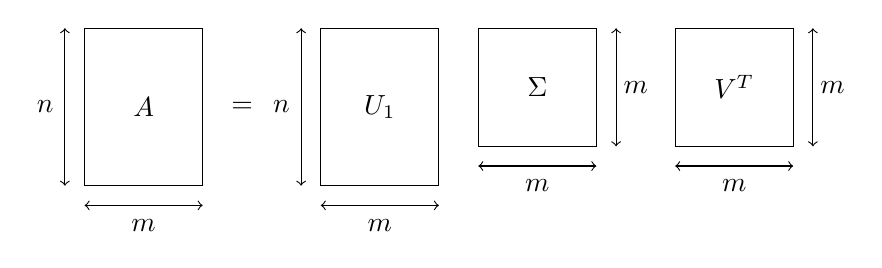
\begin{tikzpicture}
	\draw (0,0) rectangle (1.5, 2);
	\node at (0,0) {};
	\draw [<->] (-0.25,2) -- (-0.25,0);
	\draw [<->] (0,-0.25) -- (1.5,-0.25);
	\node at (2,1) {=};
	\draw (3,0) rectangle (4.5,2);
	\draw [<->](2.75,2) -- (2.75,0);
	\draw [<->] (3,-0.25) -- (4.5,-0.25);
	\draw (5,2) rectangle (6.5,0.5);
	\draw (7.5,2) rectangle (9,0.5);
	\draw [<->] (5,0.25) -- (6.5,0.25);
	\draw [<->]  (6.75,2) -- (6.75,0.5);
	\draw [<->] (7.5,0.25) -- (9,0.25);
	\draw [<->]  (9.25,2) -- (9.25,0.5);
	\node at (0.75,1) {$A$};
	\node at (3.75,1) {$U_1$};
	\node at (5.75,1.25) {$\Sigma$};
	\node at (8.25,1.25) {$V^T$};
	\node at (-0.5,1) {$n$};
	\node at (0.75,-0.5) {$m$};
	
	\node at (2.5,1) {$n$};
	\node at (3.75,-0.5) {$m$};
	\node at (5.75,0) {$m$};
	\node at (7,1.25) {$m$};
	\node at (8.25,0) {$m$};
	\node at (9.5,1.25) {$m$};
\end{tikzpicture}

\[
	A = U_1 \cdot \Sigma_1 \cdot V^T 
\]

Dla każdej macierzy $A \in \RR^{n, m}$ istnieje rozkład:
\begin{itemize}
  \item $U_1^TU_1 = \eye$ (kolumny $U_1$ są ortogonalne)
  \item $V^TV = I$
\end{itemize}

\[
\Sigma_1 = \left[\begin{array}{cccc} \sigma_1 & & & \text{\huge 0} \\
 & \sigma_2 & & \\ & & \ddots & \\ \text{\huge 0} & & & \sigma_n \end{array}\right]
\]

$\sigma _{i}$ - nieujemne wartości szczególne (osobliwe) macierzy A, uporządkowane nierosnąco ($\sigma_{i} \geq 0$).

kolumny $U_1$ - lewe wektory szczególne

kolumny $V$ - prawe wektory szczególne

\textbf{Wariant ``pełny" rozkładu SVD:}

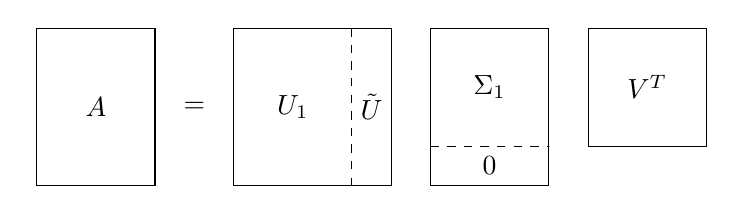
\begin{tikzpicture}
	\draw  (0,0) rectangle (1.5, 2);
	\node at (0,0) {};
	\node at (2,1) {=};
	\draw  (2.5,0) rectangle (4.5,2);
	\draw  (5,2) rectangle (6.5,0);
	\draw  (7,2) rectangle (8.5,0.5);
	\node at (0.75,1) {$A$};
	\node at (3.25,1) {$U_1$};
	\node at (5.75,1.25) {$\Sigma_1$};
	\node at (7.75,1.25) {$V^T$};
	\draw [dashed] (5,0.5) -- (6.5,0.5);
	\draw [dashed] (4,2) -- (4,0);
	\node at (5.75,0.25) {$0$};
	\node at (4.25,1) {$\tilde{U}$};
\end{tikzpicture}

\begin{fakt} $\ $ %todo usunąć ten hack na nową linjkę :D
	\begin{enumerate}
		\item Jeśli $A=A^T$, to oczywście ma rozkład $A = U \cdot \Lambda \cdot U^T$, gdzie kolumny $U$ to wartości własne A, $\Delta = \begin{bmatrix}
		      \lambda_1 & 0 & 0\\ 
		      0 & \ddots & 0\\ 
		      0 & 0 & \lambda_n 
		\end{bmatrix}$, gdzie $\lambda_i$ - wartość własna A.
		
		Wtedy SVD dla A to:
		$A = U\Sigma V^T$, gdzie $\sigma_i = |\lambda_i|$, $v_i = sign(\lambda_i)u_i$
		 			
		\item Wartość własna $A^TA$ to $\sigma_i^2$.
		       			
		      Dowód: $A^TA = (U_1\Sigma V^T)^T(U_1 \Sigma_1 V^T) = V \Sigma_1 \underbrace{U_1^T U_1 \Sigma_1 V^T}_{I} = V \Sigma_1^2V^T$, $\Sigma_1^2 = \begin{bmatrix}
		      \lambda_1^2 & 0 & 0\\ 
		      0 & \ddots^2 & 0\\ 
		      0 & 0 & \lambda_n^2 
		\end{bmatrix}$.
				
		\item $AA^T$ jej wartość własna to $\sigma_1^2, ..., \sigma_m^2$ i $(n-m)$ zer.
		      Dowód: analogicnzie jak 2.
		      		
		\item Jeśli $A$ - pełnego rzędu, to rozwiązaniem LZNK $\norm{b - AX}_2 \ra min!$ jest $x = V\Sigma_1^{-1} U_1^Tb$.
		      		
		      Dowód:
		      \[
		      	\norm{b - U\Sigma V^Tx} _2 ^2 = \norm{U(U^Tb - \Sigma V^Tx)}_2^2 = \norm{U^Tb - \Sigma V^Tx}_2^2 =
		      	\]
		      	
		      	\[\arraycolsep=1em\def\arraystretch{2} = \norm{\left[\begin{array}{c}
		      	U_1^Tb\\ 
		      	\hline
		      	\tilde{U}^Tb
		      	\end{array}\right] - \left[\begin{array}{c}\Sigma_1V^Tx\\ \hline 0 \end{array}\right]}_2^2 = \norm{\left[\begin{array}{c}U_1^Tb - \Sigma_1V^Tx\\ \hline \tilde{U}^Tb \end{array}\right]}_2^2 =\norm{U_1^Tb - \Sigma_1V^Tx\norm{_2^2 +} \tilde{U}^Tb}_2^2
		      \]
		      
		      x spełniający równanie:
		      \[
		      	\Sigma_1V^Tx = U_1^Tb
		      \]
		      
		      zeruje pierwszy składnik (czyli jak rozwiązanie LZNK)
	\end{enumerate}
\end{fakt}

\subsection{Nieregularne zadanie najmniejszych kwadratów}

Niech $A \in \RR^{m \times n}$, $n \geq m$, ale $rank(A) < m$.

Wtedy LZNK ma niejednoznaczne rozwiązanie.

Jeśli x minializuje $\norm{b - Ax}_2$, to $x+v$ też, o ile $v \in ker(A)$:

\[
	\norm{b - A(x + v)}_2 = \norm{b - Ax - \underbrace{Av}_{=0}}_2 = \norm{b - Ax}_2
\]

Dodając do zadania dodatkowy warunek, że $x$ ma mieć najmniejszą normę $\norm{\cdot}_2$ wśród wszystkich $x$ minimalizujących $\norm{b - Ax}_2$, dostajemy zadanie jednoznaczne: można je rozwiązać, korzystając z SVD!

Ponieważ A jest rzędu $k<m$, to 

\[
	\Sigma_1 = \left[ \begin{array}{ccc|ccc}
		\sigma_1 &  &  &  &  & \\ 
		&  \ddots &  &  & 0  & \\ 
		&  & \sigma_k  &  &  & \\ 
		\hline
		&  & &  0 &  & \\ 
		&  0 &  &  & \ddots & \\ 
		&  &  &  &  & 0
	\end{array} \right]
\]
$\sigma_1 \geq \cdots \geq \sigma_k > 0$.

Zatem

\[\arraycolsep=1em\def\arraystretch{2}
	\left[\begin{array}{c} \\ A \\ \ \end{array}\right] =
	\left[\begin{array}{c|c|c} & &\ \\ \tilde{U}_1 & \hat{U}_1 & \tilde{U} \\ & & \ \end{array}\right] \cdot \left[ \begin{array}{c} \begin{array}{c|c} \tilde{\Sigma}_1 & 0 \\ \hline 0 & 0 \end{array} \\ \hline 0\end{array}\right] \cdot \left[ \begin{array}{c} \tilde{V}_1^t \\ \hline \tilde{V}_2^T \end{array}\right] = \tilde{U}_1 \tilde{\Sigma}_1 \tilde{V}_1^T
\]

Postępując analogicznie jak w 4.

\[\arraycolsep=1em\def\arraystretch{2}
\norm{b - Ax}_2^2 = \norm{\left[ \begin{array}{c}
\tilde{U}_1^T \\ \hline
\hat{U}_1^T \\ \hline
\tilde{U}^T 
\end{array}\right] (b - \tilde{U}_1 \tilde{\Sigma}_1 \tilde{V}_1^Tx)}_2^2 = \norm{\left[\begin{array}{c}
\tilde{U}_1^Tb - \tilde{\Sigma}_1\tilde{V}_1^Tx \\ \hline
\hat{U}_1^T b\\ \hline
\tilde{U}^T b 
\end{array}\right]}_2^2 = 
\norm{\tilde{U}_1^Tb - \tilde{\Sigma}_1\tilde{V}_1^Tx}_2^2 +  \norm{\hat{U}_1^Tb}_2^2 + {\hat{U}^Tb}_2^2
\]

Minimum tego wyrażenia dla $x = \tilde{V}_1\tilde{\Sigma}_1^{-1} \tilde{U}_1^Tb$.

Inne rozwiązania są postaci $x+v$, gdzie $v \in ker(A)$. Ponieważ $v \in ker(A)$ jest postaci $v = \tilde{V}_2 \cdot z$ dla pewnego z.

$\norm{x + v}_2^2 = \norm{x}_2^2 + \norm{v}_2^2$, gdyż $x \bot v$

$x^Tv = (\tilde{V_1} \cdot cos)^T) (\tilde{V}_2z) = cos^T \cdot \underbrace{\tilde{V}_1^T\tilde{V}_2}_{=0}\cdot z = 0$, więc $\norm{x + v}_2$ najmniejsza gdy $v = 0$.

\subsection{Uwarunkowanie LZNK}

$A \in \RR^{n,m}$, $n \gg m$, $rank(A) = m$, $r$ - rozwiązanie LZNK $\norm{b - Ax}_2 \ra min!$

Rozważmy zadanie zaburzone

\[\norm{\tilde{b} - \tilde{A}\tilde{x}}_2 \ra min\]

Załóżmy, że

\[
	\varepsilon := max \left\{ \cfrac{\norm{A - \tilde{A}}_2}{\norm{A} _2}, \cfrac{\norm{b - \tilde{b}}_2}{\norm{b}_2} \right\}
\]

jest na tyle małe, że $cond_2(A) \cdot \varepsilon < 1$, gdzie $cond_2(A) := \cfrac{\sigma_{max}(A)}{\sigma_{min}(A)}$.

Wtedy zadanie zauburzone ma jednoznaczne rozwiązanie oraz $cond_{LZNK}(A, b)$:

\[
	\cfrac{\norm{x - \tilde{x}}_2}{\norm{x}_2} \leq \varepsilon \cdot \underbrace{\left[ \cfrac{2 cond_2(A)}{\cos{\Theta}} + \tan{\Theta}(cond_2(A))^2 \right]}_{cond_{LZNK}(A, b)} + O(\varepsilon^2)
\]

gdzie $\sin{\Theta} = \cfrac{\norm{b - Ax}_2}{\norm{b}_2}$

Zatem:

\begin{enumerate}
	\item $\sin\Theta \simeq$ (tzn. residuum jest małe), wtedy $cond_{LZNK}(A, b) \simeq K cond_2(A)$.
	      	
	\item $\sin\Theta \simeq 1$ (tzn. x jest bliskie zera i duże residuuum!), wtedy $cond_{LZNK}(A, b)\gg 1$ nawet jeśli $cond_2(A) \simeq 1$
	      	
	\item wpp. $cond_{LZNK} \simeq K \cdot cond_2^2(A)$
\end{enumerate}

\section{Zagadnienie własne}

$A \in \RR^{n \times n}$: $(\lambda, v) \in \CC \times \CC^n$ jest parą własną, tzn.

\[
	Av = \lambda v
\]

oraz $v \neq 0$. Jeśli $A = A^T$, to wszystkie warotści własne i wektory wlasne są rzeczywiste i tworzą bazę ortogonalną:
\[
	Q^TAQ = \Lambda = \left[\begin{array}{ccc}
	\lambda_1 &  & \\ 
	&  \ddots & \\ 
	&  & \lambda_n
	\end{array}\right]
\]

gdzie

\[
	Q = \left[ \begin{array}{c|c|c|c} & & & \\ v_1 & v_2 & \cdots & v_n \\ & & & \end{array} \right]
\]

gdzie $Q^TQ = I$.

Typowe zadania obliczeniowe:

\begin{itemize}
	\item znaleźć ekstremalne wartości własne (lub wektory własne im odpowiadające)
	\item znaleźć wartości własne bliskiej zadanej liczbie (lub ...)
	\item znaleźć wszystkie wartości własne (i wektory).
\end{itemize}

\subsection{Metoda potęgowa}
Czyli wyznaczanie wektora własnego odpowiadające dominującej wartości własnej

Niech wartości własne A spełniają:

\[
	|\lambda_1| \underbrace{>}_{\textrm{tak, tu ostra}} |\lambda_2| \geq |\lambda_3| \geq \cdots \geq |\lambda_n|
\]

Algorytm:

for k = 0, 1, ...
 
$x_{k+1} = A \cdot x_k$

$x_{k+1} = \cfrac{x_{k+1}}{\norm{x_{k+1}}_2^2}$

end
 
Działanie tej metody przeanalizujemy dla A, która jet diagonalizowalna:
 
\[
	X^{-1} A X = \Lambda = \begin{bmatrix} \lambda_1 &  & \\  &  \ddots & \\ &  & \lambda_n \end{bmatrix}
\]
 
Innymi słowy:
 
\[
	AX = X \Lambda
\]
 
czyli kolumny $v_i$, macierzy X:
 
$X = \left[ \begin{array}{c|c|c|c} &&& \\ v_1 & v_2 & \cdots & v_n \\ &&& \end{array} \right]$ są wektorami własnymi odpowiadającymi $\lambda_i$.
 
Zapisując $x_0 = \sum_{i=1}^{n} \alpha_i v_i$ mamy kolejno:
 
\begin{align*}
	x_1 & = A \cdot x_0 = A \sum \alpha_iv_i = \sum \alpha_i Av_i = \sum \alpha_i \lambda_i v_i \\
	x_2 & = Ax_1 = A(\sum(\alpha_i\lambda_i)\cdot v_i) = \sum \alpha_i \lambda_i^2 v_i \\
	& \vdots \\
	x_k & = \sum \alpha_i \lambda^k v_i \\ & = \lambda_1^k\left(\alpha_1 v_1 + \alpha_2\underbrace{(\cfrac{\lambda_2}{\lambda_1})^k}_{| \cdots | < 1 \ra 0} v_2 + \cdots + \alpha_n \underbrace{(\cfrac{\lambda_n}{\lambda_1})^k}_{| \cdot | < 1 \ra 0} \cdot v_n\right)
\end{align*}
 
Szybkość zbieżności $x_k$ do kierunku wektora $v_1$ jest proporcjonalna do $\left| \cfrac{\lambda_2}{\lambda_1} \right| < 1$.
 
% powtorzenie wykladu
%Zadanie własne $A \in \RR^{N\times N}$:
%
%\[
%	(\lambda, x) \in \CC \times \CC^N \quad Ax = \lambda \cdot x
%\]

%Co warto zauważyć:

\begin{fakt}
	Jeśli $\lambda$ - w. własna macierzy A, to $(\lambda - \nu)$ - w. własny macierzy $(A - \nu I)$
	 
	\[
		(A - \nu I)v \overbrace{=}^{v\textrm{ - wektor własny odpowiadający }\lambda} = Av - \lambda v = \lambda v - \nu v = (\lambda - \nu)v
	\]
\end{fakt} 

\begin{fakt} Jeśli $\lambda$ - wartość własna A oraz A - nieosobliwa, to $\cfrac{1}{\lambda}$ jest wartością własną $A^{-1}$.
	
	\begin{equation}
		\begin{aligned}
			A^{-1}| Av           & = \lambda v                                  \\
			v                    & = A^{-1}(\lambda v) = \lambda \cdot A^{-1} v \\
			\cfrac{1}{\lambda} v & = A^{-1}v                                    
		\end{aligned}
	\end{equation}
	
\end{fakt}

\begin{fakt} Jeśli $\lambda$ - wartość własna A oraz $(A - \nu I)$ - nieosobliwa, to $\cfrac{1}{\lambda - \nu}$ jest wartością własną $(A - \nu I)^{-1}$
\end{fakt}

\begin{wniosek} Metoda potęgowa zastosowana do $(A - \nu I)^{-1}$ będzie zbieżna do wartości własnej A, $\lambda_i$, najbliższej $\nu$ (jeśli taka jedyna $\lambda_i$ istnieje). Rzeczywiście, wartość własna $(A - \nu I)^{-1}$ to $\cfrac{1}{\lambda - \nu}$, jeśli zachodzi $\cfrac{1}{|\lambda_i - \nu|} > \cfrac{1}{|\lambda_j - \nu|}$ dla $j \neq i$, to $\cfrac{1}{|\lambda_i - \nu|}$ jest dominująca.
\end{wniosek}

[dotąd ma być kolos]

\subsection{Odwrotna metoda potęgowa}

for k = 0, 1, 2...
 
$x_{k+1} = (A - \nu I)^{-1}\cdot x_k$
 
$x_{k+1} = \cfrac{x_{k+1}}{\norm{x_{k+1}}}$


Ten algorytm w praktyce oczywiście implementujemy inaczej.

$O(N^3) \ra $ Rozłóż macierz na czynniki, np. $P(A-\nu I) = LU$ (albo $A - \nu I = QR$)

1. for k = 0, 1, 2, ... 

2. rozwiąż układ $Ly = (Px_k)$

3. rozwiąż układ $U x_{k+1} = y$

4. $x_{k+1} = \cfrac{x_{k+1}}{\norm{x_{k+1}}}$

---

(2 i 3 - $O(n^2)$)

---

Znając przybliżenie $x_k$ wektora własnego, możemy wykonać najlepsze (w sensie średniokwadratowym) przybliżenie wartości własnej:

\[
	\lambda_k = \underbrace{\cfrac{x^T_k A x_k}{x_k^T x_k}}_{\textrm{iloraz Rayleigh}}
\]

(gdy $x_k \in \CC^N$, $\cfrac{x_k^H A x_k}{x_k^Hx_k}$)

Gdy $x_k = v$: $\cfrac{v^TAv}{v^Tv} = \cfrac{v^T \lambda v}{v^T v} = \lambda \cdot \cfrac{v^T v}{v^T v} = \lambda$


\textbf{Metoda Rayleigh:}

for k = 0, 1, 2...

Rozwiąż $(A - \nu_k I)x_{k+1} = x_k \quad \la O(N^3)$
 
$x_{k+1} = \cfrac{x_{k+1}}{\norm{x_{k+1}}}$

$\nu_{k+1} = x_{k+1}^T A x_{k+1}$
 
Ale ta metoda ma problem, bo coś tam psujemy macierz jak się zmienia wartość własna. Złe uwarunkowanie tej macierzy tylko nam pomaga, a nie przeszkadza! Dlaczego? Dlatego, że ta macierz robi się coraz bardziej źle uwarunkowana, więc $x_k$, który liczymy coraz mniej przypomina prawdziwy $x$. Rozwiązanie jest obarczone coraz większym błędem, ALE! Cały ten błąd jest skierowany w stronę naszego wektora własnego. Czyli otrzymujemy jeszcze lepszy $x$ niż normalnie. Czyli dobrze jest, dobrze! (no prawie, jak źle zaczniemy, to ta pierwsza iteracja może nas wrzucić w okolice innej wartości własnej). 


\subsection{Wartości własne macierzy blokowo-trójkątnej:}

Jeśli $A = \left[\begin{array}{c|c}A_{11} & A_{12} \\ \hline 0 & A_{22}\end{array}\right]$, gdzie $A_{11}$, $A_{22}$ - macierze kwadratowe, to

$\underbrace{\sigma(A)}_{\textrm{spektrum, czyli zbiór wartości własnych A}} = \sigma(A_{11}) \cup \sigma(A_{22})$

Rzeczywiście $\lambda$ jest wartością własną $A$ $\iff det(A -\lambda I) = 0$.

No dobrze, ale ile wynosi wyznacznik?

\begin{equation}
	\begin{aligned}
		det(A - \lambda I) & = det\left( \left[\begin{array}{c|c}A_{11} & A_{12} \\ \hline 0 & A_{22}\end{array}\right] - \lambda  \left[\begin{array}{c|c}I & 0 \\ \hline 0 & I\end{array}\right] \right) \\
		& = det\left( \left[\begin{array}{c|c}A_{11}-\lambda I & A_{12} \\ \hline 0 & A_{22} - \lambda I\end{array}\right]\right) \\
		& = det(A_{11} - \lambda I) \cdot det(A_{22} - \lambda I)
	\end{aligned}
\end{equation}

\textbf{Fakty w lokalizacji wartości własnych:}

\begin{fakt}
	Jeśli $\lambda$ - wartość własna A, to $|\lambda| \leq \norm{A}$.
		
	Istotnie, dla $v$ - wektor własny A odpowiadając wartości własnej $\lambda$,
		
	\begin{equation}
		\begin{aligned}
			Av             & =\lambda v                                                                                   \\
			\norm{A v}    & = \norm{\lambda v} = |\lambda| \cdot \norm{v}                                              \\
			\textrm{stąd} &                                                                                              \\
			|\lambda|      & = \cfrac{\norm{A v}}{\norm{v}} \leq sup_{x \neq 0} \cfrac{\norm{Ax}}{\norm{x}} = \norm{A} 
		\end{aligned}
	\end{equation}
		
\end{fakt}

\begin{twierdz}[Goershgorina] $\sigma(A)$ jest zawarte w sumie teoriomnogościowej tzw. kół Gershgerina
	
	\[
		K_{i} := \left\{ z \in \CC: |z - a_{ii} | \leq \sum_{j \neq i} |a_{ij}| \right\}
	\]
	
	(???jak daleko liczby z diagonali wyznaczają wartości własne???)
	
	\begin{tikzpicture}
		
		
		\draw [->] (-5,0) -- (5,0);
		\draw [<-] (0,2) -- (0,-2);
		\draw  (-2.5,0) circle (1);
		\draw  (0.5,0) circle (1.4);
		\draw  (3,0) circle (0.7);
	\end{tikzpicture}
	
	Dowód pomijam, bo dowód.
	
\end{twierdz}

\begin{twierdz}[o uwarunkowaniu zadania wyznaczania wartośći własnej macierzy diagonalizowalnej, twierdzenie B....?-Fike]
	Niech $A$ będzie diagonaliziwalna, tzn. istnieje $X$ nieosobliwa t. że
	
	\[
		X^{-1}AX = \left[ \begin{array}{ccc} \lambda_i & & \\ & \ddots \\ & & \lambda_N \end{array} \right] = \Lambda
	\]
\end{twierdz}

Niech $\tilde{\lambda}$ - w. własna macierzy zaburzonej $\tilde{A} = A + \Delta$. Wtedy

\[
	min_{\lambda \in \sigma(A)} |\lambda - \tilde{\lambda} \leq \underbrace{\norm{X} _2 \cdot \norm{X^{-1}}_2}_{cond_2(X)} \cdot \norm{\Delta}_2
\]

\begin{fakt}Jeśli $\norm{M} < 1$, to macierz $\II+M$ jest nieosobliwa.
\end{fakt}

\begin{wniosek}
	Jeśli $A$ - symetryczna, to $min_i |\lambda_i - \tilde{\lambda}| \leq \norm{\delta}_2$
	
	Dowód: Wynika stąd, że $Q^TAQ = \Lambda$, gdzie $Q$ - macierz ortogononalna: $Q^TQ = I$. Zatem $cond_2(Q) = 1$.
\end{wniosek}

\subsection{Metoda QR wyznaczania wszystkich wartości własnych macierzy}

Algorytm w wersji najprostszej:

$A_1 = A$

for k = 1, 2, ....

$\quad A_k =: Q_kR_k$ (wyznacz rozkład QR)
 
$\quad A_{k+1} := R_kQ_k$ (przemnoż go w drugą stronę)

I to już cała iteracja.

Po pierwsze zauważmy, że $A_k$ mają to samo spektrum, co macier $A$. No rzeczywiście, bo 

\begin{equation}
	\begin{aligned}
		A_{k+1} & = R_kQ_k                            \\
		        & = Q_k^T\underbrace{Q_kR_k}_{A_k}Q_k \\
		        & = Q_k^TA_kQ_k = ...                 \\
		        & = Q_k^T\cdots Q_1^TA Q_1 \cdots Q_k 
	\end{aligned}
\end{equation}

W ogólnym przypadku może wolno działać (nie być zbieżna, wolno zbieżna). Dlatego powstaje pytanie jak ulepszyć tę metodę? 

\textbf{Ulepszenia metody QR i przesunięcia}

Najprostsze takie ulepszenie:

$A_1 = A$

for k = 1, 2, ....

$\quad$ wybierz przesunięcie $\sigma_k$

$\quad A_k =: Q_kR_k = A_k - \sigma_k I $ (wyznacz rozkład QR i przesuń)
 
$\quad A_{k+1} := R_kQ_k + \sigma_k I$ (przemnoż go w drugą stronę i przesuń)

\textbf{Praktyczne QR:}

Teraz ten algorytm jest niepraktyczny. Ile kosztuje rozkład QR? Jak macierz jest jakakolwiek, to oczywiście $O(N^3)$. Co zrobić żeby ten algorytm był praktyczny? Przed rozpoczęciem iteracji należy sprowadzić macierz przekształceniami ortogoalnymi do postaci Hessenberga: $\left[ \begin{array}{cccc} \star & \cdots & \star \\ \star & \ddots & \vdots \\ 0 & \ddots \\  \end{array} \right]$, a gdy A jest symetryczna, tzn. $A=A^T$, to do postaci symetrycznej Hessenberga (trójdiagonalnej). Ostatecznie dobrze zaimplementowana metoda QR kosztuje $O(N^3)$.

\end{document}
